

%\documentclass[a4paper]{jarticle}

\section{mbar.rb 棒グラフの描画\label{sect:mbar}}
\index{mbar@mbar}

棒グラフを描画するコマンドである。
x軸・y軸に展開する属性項目を指定することで、
1次元もしくは2次元の棒グラフ行列を描画することができる。
グラフは単独のHTMLファイルとして出力されるので、
一般的なブラウザで表示が可能である。

入力データには、表\ref{tbl:mbar_input2}のようなCSVを用いる。
棒グラフを構成する項目を構成要素項目といい、
\verb|f=|パラメータで指定する。
x軸・y軸に展開する属性項目は\verb|k=|パラメータで指定する。
\verb|k=|パラメータで1項目を指定すると1次元の(x軸に展開された)棒グラフ行列が、
2項目を指定すると2次元の(x軸・y軸に展開された)棒グラフ行列が描画される。
\verb|k=|パラメータを省略した場合は、1個の棒グラフが描画される。

なお棒グラフの描画には、内部的に
JavaScriptライブラリD3.js(Data-Driven Documents)を使用している。
D3.jsの詳細は公式ページ(\url{http://d3js.org/})を参照のこと。

また本コマンドを利用するためには、nysol/mcmdライブラリが必要となる。

\begin{table}[http]
\begin{center}
\caption{都道府県と年代別の個体数\label{tbl:mbar_input2}}
{\small
\begin{tabular}[t]{ccr}
\hline
Pref&Age&Population \\
\hline
奈良&10&310504\\
奈良&20&552339\\
奈良&30&259034\\
奈良&40&450818\\
奈良&50&1231572\\
奈良&60&1215966\\
奈良&70&641667\\
北海道&10&310504\\
北海道&20&252339\\
北海道&30&859034\\
北海道&40&150818\\
北海道&50&9231572\\
北海道&60&4215966\\
北海道&70&341667\\
\hline
\end{tabular}
}
\end{center}
\end{table}

\newpage
\subsection{書式}
\begin{verbatim}
  mbar.rb [i=] f= v= [o=] [k=] [title=] [width=] [height=] [cc=] [--help]
\end{verbatim}

\begin{table}[htbp]
{\small
\begin{tabular}{ll}
\verb|i=|        & 入力データファイル名(CSV形式)\\
\verb|f=|        & 構成要素項目名を指定する。\\
                 & データにnullが含まれる場合は無視する。\\
\verb|v=|        & 構成量項目(棒グラフの高さを決定する項目)を指定する。\\
                 & データにnullが含まれる場合は0として扱う。\\
                 & マイナス、小数点に対応している。\\
                 & 先頭の0は無視する。数字以外の場合はエラーとなる。\\
\verb|o=|        & 出力ファイル名(HTMLファイル)\\
\verb|k=|        & x軸・y軸に展開する属性項目名を2つ以内で指定する。\\
                 & 省略した場合は棒グラフを1つ作成する。\\
                 & 項目を1つ指定した場合は1次元の棒グラフ行列を、\\
                 & 項目を2つ指定した場合は2次元の棒グラフ行列を作成する。\\
\verb|title=|    & グラフのタイトル文字列を指定する。\\
\verb|width=|    & 棒グラフ用描画枠の横幅を指定する(デフォルトは250、1つの棒グラフは600)。\\
\verb|height=|   & 棒グラフ用描画枠の縦幅を指定する(デフォルトは250、1つの棒グラフは400)。\\
\verb|cc=|       & 1行に表示する棒グラフの最大数を指定する(デフォルトは5)。\\
                 & 1次元の棒グラフ行列のときのみ指定できる。\\
\verb|--help|    & ヘルプの表示\\
\end{tabular} 
}
\end{table} 

なお\verb|mbar.rb|コマンドには、
\verb|f=|パラメータや\verb|k=|パラメータで指定した項目を
自動的に並べ替える機能はない。
グラフに表示したい順に、あらかじめ並べ替えておく必要がある。

\subsection{利用例}
\subsubsection*{例1: Basic Example}

Using the data \verb|dat1.csv|, set \verb|Age| as the unit of composition, draw a one dimensional bar graph showing the population.
The output of the bar chart can be viewed in the web browser. Note that in the bar chart, when you place the mouse cursor over the bar chart, details of the unit of composition is shown in a pop-up box. The graph can also be moved by dragging the mouse, and the size of the graph can be scaled by scrolling the mouse.


\begin{Verbatim}[baselinestretch=0.7,frame=single]
$ more dat1.csv
Age,Population
10,310504
20,552339
30,259034.5555
40,0450818
50,1231572
60,1215966
70,641667
$ mbar.rb i=dat1.csv v=Population f=Age o=result1.html
#END# /usr/bin/mbar.rb i=dat1.csv v=Population f=Age o=result1.html
$ head result1.html
<!DOCTYPE html>
<html>
<head>
<meta charset="utf-8">
<style>
body {
  font: 10px sans-serif;
}
\end{Verbatim}

\begin{flushleft}
\fbox{
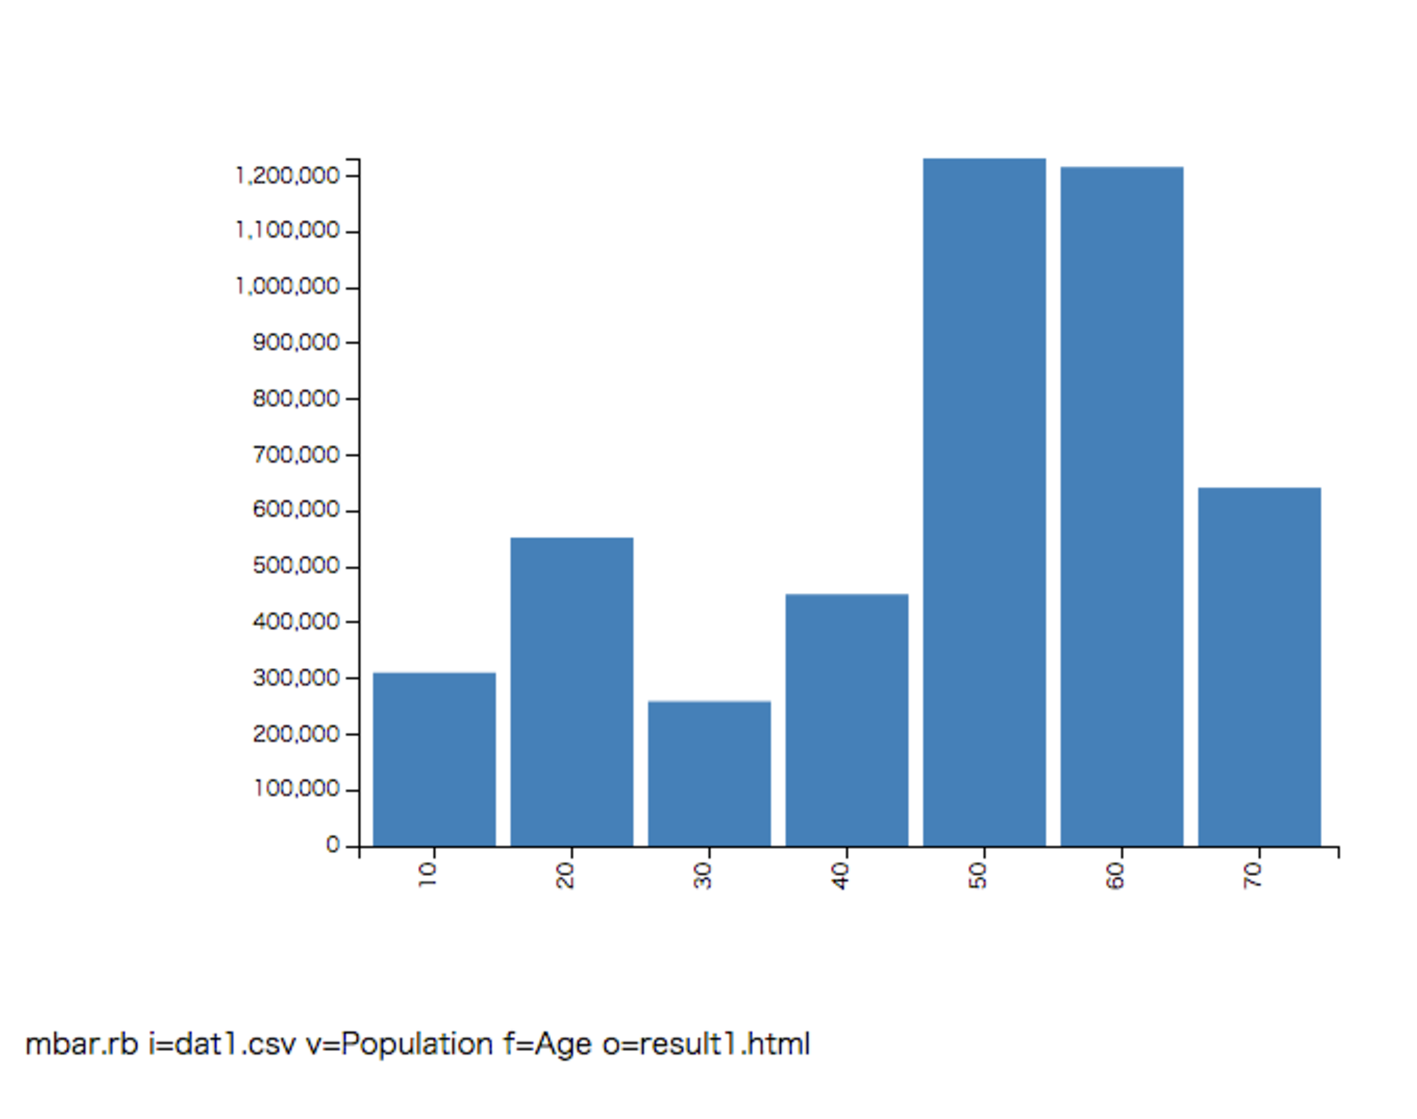
\includegraphics[scale=0.5]{figure/mbar1.eps}
}
\end{flushleft}

\subsubsection*{例2: Draw a one dimensional bar graph matrix}

Using the data \verb|dat2.csv|, set \verb|Age| as the unit of composition, draw the bar graph showing the population. Specify \verb|Pref| at ¥verb|k=| parameter, which designates pref on the x-axis, extended horizontally as a one-dimensional bar graph. Specify the title of the graph at \verb|title=| parameter.


\begin{Verbatim}[baselinestretch=0.7,frame=single]
$ more dat2.csv
Pref,Age,Population
Nara,10,310504
Nara,20,552339
Nara,30,259034
Nara,40,450818
Nara,50,1231572
Nara,60,1215966
Nara,70,641667
Hokkaido,10,310504
Hokkaido,20,252339
Hokkaido,30,859034
Hokkaido,40,150818
Hokkaido,50,9231572
Hokkaido,60,4215966
Hokkaido,70,341667
$ mbar.rb i=dat2.csv k=Pref v=Population f=Age o=result2.html title='Population of Nara and Hokkaido by Age Group'
#END# /usr/bin/mbar.rb i=dat2.csv k=Pref v=Population f=Age o=result2.html title='Population of Nara and Hokkaido by Age Group'
$ head result2.html
<!DOCTYPE html>
<html>
<head>
<meta charset="utf-8">
<style>
body {
  font: 10px sans-serif;
}
\end{Verbatim}

\begin{flushleft}
\fbox{
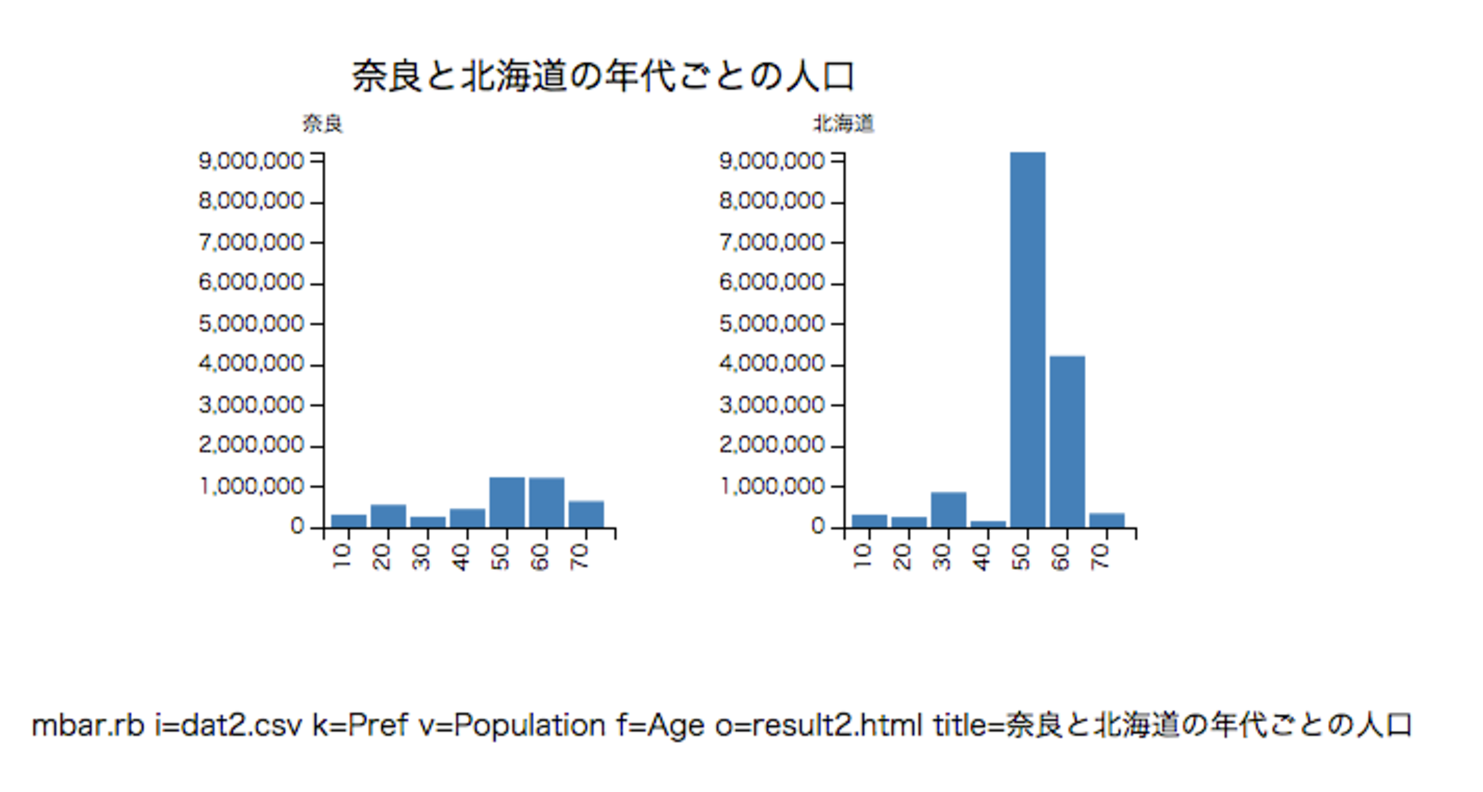
\includegraphics[scale=0.5]{figure/mbar2.eps}
}
\end{flushleft}


\subsubsection*{例3: Draw a two dimensional bar graph matrix}

Using the data \verb|dat3.csv|, set \verb|ThemePark| as the unit of composition, draw the bar graph showing the number item, and set the \verb|width=| at 200, and \verb|height=| at 150. Specify \verb|Gender| and \verb|Age| at \verb|k=| parameter, which designates Gender on the x-axis extended horizontally, and Age on y-axis extended vertically.


\begin{Verbatim}[baselinestretch=0.7,frame=single]
$ more dat3.csv
Gender,Age,ThemePark,Number
Male,30,Disney,100
Male,30,UFJ,59
Male,30,Umeyashiki,180
Male,40,Disney,200
Male,40,UFJ,3
Male,40,Umeyashiki,10
Male,50,Disney,110
Male,50,UFJ,40
Female,30,Umeyashiki,100
Female,30,Disney,80
Female,30,UFJ,200
Female,40,Disney,90
Female,40,UFJ,80
Female,40,Umeyashiki,120
Female,50,Disney,99
Female,50,UFJ,80
Female,50,Umeyashiki,110
$ mbar.rb i=dat3.csv k=Gender,Age v=Number f=ThemePark o=result3.html
#END# /usr/bin/mbar.rb i=dat3.csv k=Gender,Age v=Number f=ThemePark o=result3.html
$ head result3.html
<!DOCTYPE html>
<html>
<head>
<meta charset="utf-8">
<style>
body {
  font: 10px sans-serif;
}
\end{Verbatim}

\begin{flushleft}
\fbox{
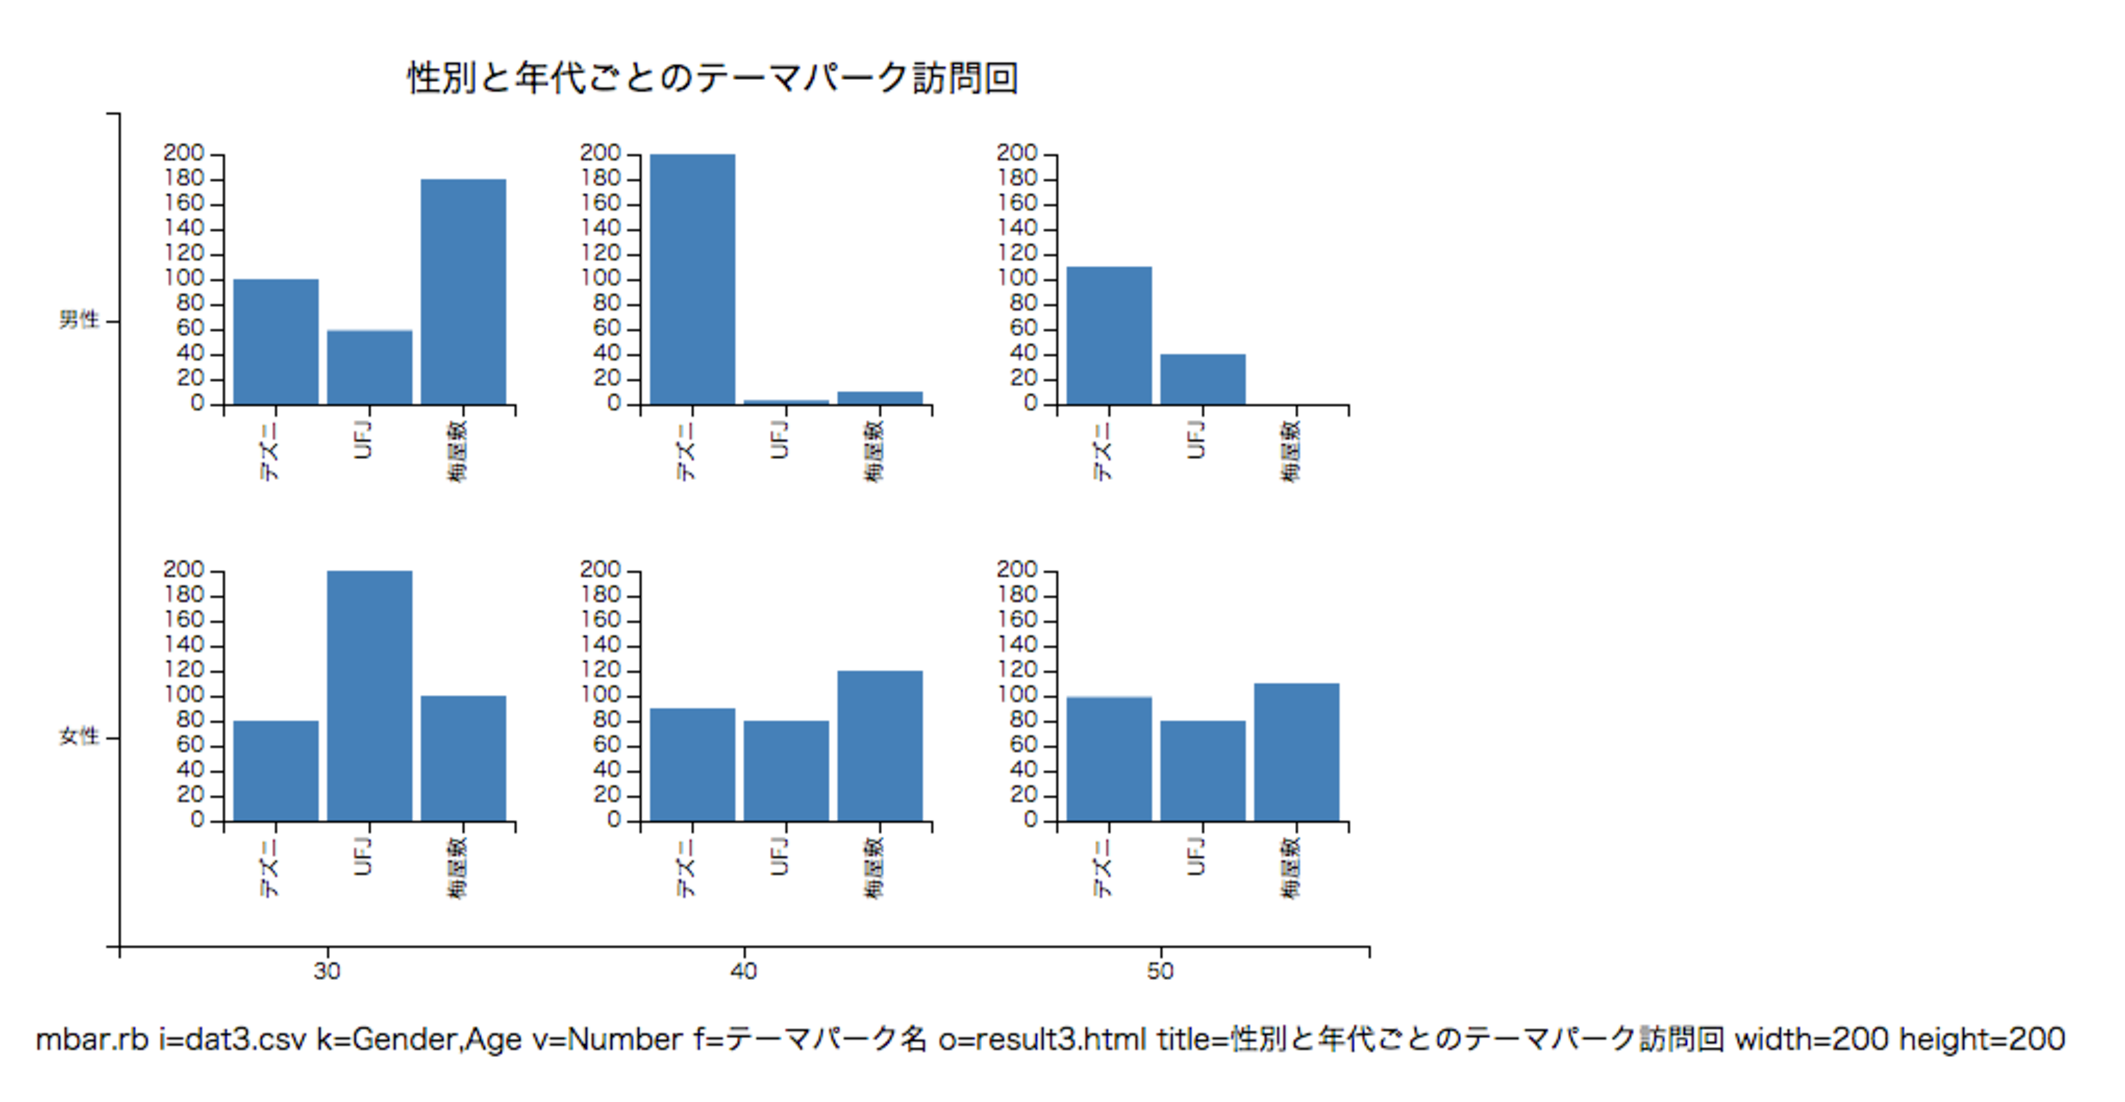
\includegraphics[scale=0.5]{figure/mbar3.eps}
}
\end{flushleft}



%\end{document}

